\label{app4}





\section{Simplified Inverse Kinematics}

The controller demands that the configuration of the actuator is known at each sampling instant. Therefore the modal coordinates need to be calculated based on the sensor data. Since the configuration of the actuator is approximated with a single shape function. The inverse kinematic problem can implicitly be solved with the constant curvature approach. The sensor output, which is the x,y position in the plane, and the orientation of the tip of the actuator $\theta$ can be used to determine modal coordinates $\epsilon$ and $\kappa$. At each sampling instant this inverse kinematics are determined. Based on the modal coordinates the Jacobian matrix can be updated, which in its turn is used in determining the new control input. The simplified kinematics are shown in Figure \ref{fig:simpkin}.

\begin{figure}[H]
    \centering
    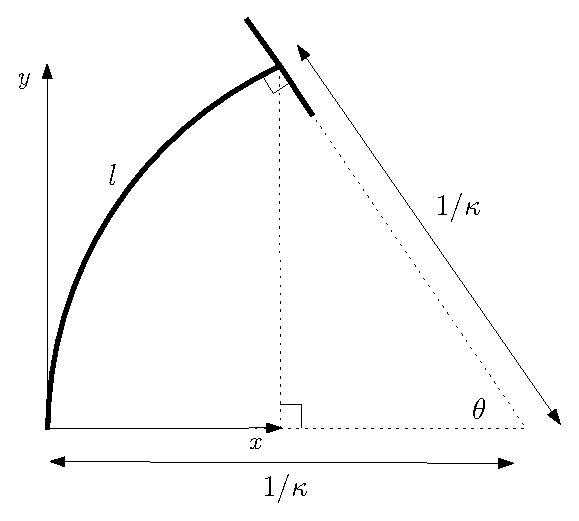
\includegraphics[width = 0.5\textwidth]{Figures/Chapter5/fbdkinematics.eps}
    \caption{Schematic drawing of the actuator to determine mapping from configuration space to task space}
    \label{fig:simpkin}
\end{figure}

From above figure the following forward kinematic relations follow as,


\begin{equation}
    y = \frac{1}{\kappa}\sin(\theta) \hspace{15pt} \text{and} \hspace{15pt}    x = \frac{1}{\kappa}[1-\cos(\theta)] \hspace{15pt} \text{with} \hspace{10pt}   \theta = l \kappa.
\end{equation}

where $l \in \mathbb{R}^{+}$ is the actuator length given by $l = (1+\epsilon)L_0$. Accordingly, the modal coordinates can then be calculated by,

\begin{equation}
    \kappa = \frac{\sin(\theta)}{y} \hspace{15pt} 	\land \hspace{15pt}  \kappa = \frac{1 -\cos(\theta)}{x} \hspace{15pt} \text{and} \hspace{10pt} \epsilon = \frac{\theta}{\kappa L_0} -1,
\end{equation}

where it should be noted that for small angles it is more accurate to use $\kappa$ based on the $\sin(\theta)$.


